\documentclass[conference]{IEEEtran}
\usepackage{hyperref}
\usepackage{tabularx}
\usepackage{cite}
\usepackage{graphicx}
\usepackage{algorithm}
\usepackage{listings}
\usepackage{microtype}

\lstset{
  breaklines=true,
  numbers=left,
  stepnumber=1,
  firstnumber=0,
  numberblanklines=false,
  xleftmargin=2em,
  framexleftmargin=1.5em
}
\begin{document}
\title{Towards a Faster Web\\High-performance Computing on the Browser}

\author{\IEEEauthorblockN{Matti Jokitulppo}
\IEEEauthorblockA{Aalto University\\
School of Science\\
Email: matti.jokitulppo@aalto.fi}
\and
\IEEEauthorblockN{Olavi Haapala}
\IEEEauthorblockA{Aalto University\\
School of Science\\
Email: olavi.haapala@aalto.fi}
\and
\IEEEauthorblockN{Mehrad Mohammadi}
\IEEEauthorblockA{Aalto University\\
School of Science\\
Email: mehrad.mohammadi@aalto.fi}
}
% make the title area
\maketitle

\begin{abstract}
Recently, a new standard for a fast, space-efficient bytecode format for the
  browser by the name of WebAssembly has been standardized,  and implemented by
  all the most prominent browser vendors. WebAssembly enables languages like C,
  C++ or Rust can be compiled to WebAssembly using existing tools, such as the LLVM-based Emscripten compiler.

  In this paper we attempt to benchmark WebAssembly against native JavaScript
  for various simple computational tasks. Initial results show that WebAssembly
  is very promising in terms of pure speed and efficiency. However, the
  developer tool chain and programming language integration still needs work.
  However, we believe WebAssembly and other intermediary tools like Babel are
  the future, and writing plain JavaScript for web applications will become
  more and more rare.
\end{abstract}

\section{Introduction}
Until now, programmers have had little option but to use JavaScript, or
languages that compile down to it like Elm or PureScript when writing modern
browser web applications applications. Furthermore, With the ever-increasing
advent of mobile computing devices and hybrid mobile applications, fast
browser-side code is more topical now than ever. However, the high-level,
interpreted nature of JavaScript makes performance difficult to achieve.
Besides speed, modern JavaScript frameworks and languages that compile down to
it can also lead to large bloated applications that can take up many megabytes
of bandwidth, due to JavaScript being a text-based format.

Browser vendors like Firefox and Chrome have made countless attempts at
optimizing the performance of JavaScript. Recently, a low-level byte code format
for client-side code called WebAssembly~\cite{wasmspeed} has been standardized. WebAssembly
promises to be faster to both execute and evaluate than ordinary JavaScript,
and also take less space. WebAssembly can also be written in various low-level
languages like C, C++ or Rust. Besides WebAssembly, other means of writing
performant client-side code in languages other than JavaScript includes asm.js,
which is a subset of JS that C/C++ can be compiled down to, utilizing some
well-supported performance optimizations of JavaScript that might be cumbersome
to write by hand. The main idea behind asm.js is that it’s output can be
directly converted into native code by browsers and their JavaScript run times,
without going through an expensive interpretation process. In real-world usage
scenarios, asm.js is often used as a fall-back for WebAssembly, if the end-user
browser does not support it. We will also look at doing calculations on the
GPU with WebGL, since nowadays especially newer mobile devices contain quite
capable GPUs, which are often quite underutilized in web applications.
Naturally, GPUs require a totally different mindset when designing the actual
algorithms since their operation differs fundamentally from CPUs, rendering
them sub-optimal for tasks such as graph traversal or sorting, since they cannot
be parallelized easily.

Within this paper we benchmark various different algorithms implemented in
plain JavaScript, the WebGL framework gpu.js, and C/C++ compiled to asm.js and
WebAssembly.  We then benchmark them on various different device and browser
combinations. The algorithms we use are  trivial and well understood, such that
possible subtle differences in implementation won't affect the end result. The
algorithms used are sorting an array, matrix multiplication and finding the nth
Fibonacci number. As is apparent, none of these algorithms are themselves
commonly used in the average web application, but they are used more as a
proof-of-concept for heavy computing on the browser.

As an example, the classic recursive algorithm for finding the nth Fibonacci
number, written in C++, can be seen in listing~\ref{cfibo}, The corresponding
WebAssembly byte code and asm.js output, both reassembled into a human-readable
format can be seen in listing~\ref{wasmfibo}. The main unit of both
compilation, distribution and evaluation of WebAssembly is the module, which
can be seen on line 1 of the compiled output. As is apparent, WebAssembly
byte code is a stack-machine based abstract syntax tree of sorts. Of course,
this format is not meant to be written by hand. The actual function definition
for our Fibonacci function starts on line 6. As was specified in the C++ code,
the function takes in a 32-bit integer and returns a 32-bit integer. On line 9,
we perform the \emph{i.32.ge\_s} instruction to check if the variable on the
call stack, which is the integer \emph{n} in the C++ code, is less than or
equal to one. In the WebAssembly code, the parameter \emph{n} is located at the
top of the stack. If \emph{n} is less than two, we simply get the local
variable from the stack at point \emph{\$0} and return it. Otherwise, we call
the \emph{i32.add} function on the the output of two additional calls to our
Fibonacci function.

The asm.js compiled output is actually extremely similar to what one would
write in regular, everyday JavaScript. The only two performance optimizations
made by the compiler in this particular piece of code is the casting of all the
variables into 32-bit unsigned integers by performing the bit wise OR operation
on them with 0, and using addition also when decrementing numbers from each
other.

\begin{figure*}[h]
  \begin{minipage}[t]{0.30\textwidth}
  \begin{lstlisting}[caption={Nth Fibonacci (C++)},label=cfibo, basicstyle=\scriptsize]

  int fibonacci(int n) {
    if (n <= 1) {
      return n;
    }
    else {
      return fibonacci(n - 1) + fibonacci(n - 2);
    }
  }
  \end{lstlisting}
\end{minipage}%
\begin{minipage}[t]{0.40\textwidth}
  \begin{lstlisting}[caption={Nth Fibonacci (WASM)},label=wasmfibo, basicstyle=\scriptsize]

(module
 (table 0 anyfunc)
 (memory $0 1)
 (export "memory" (memory $0))
 (export "_Z9fibonaccii" (func $_Z9fibonaccii))
 (func $_Z9fibonaccii (; 0 ;) (param $0 i32) (result i32)
  (block $label$0
   (br_if $label$0
    (i32.ge_s
     (get_local $0)
     (i32.const 2)
    )
   )
   (return
    (get_local $0)
   )
  )
  (i32.add
   (call $_Z9fibonaccii
    (i32.add
     (get_local $0)
     (i32.const -1)
    )
   )
   (call $_Z9fibonaccii
    (i32.add
     (get_local $0)
     (i32.const -2)
    )
   )
  )
 )
)
  \end{lstlisting}
\end{minipage}%
\begin{minipage}[t]{0.30\textwidth}
  \begin{lstlisting}[caption={Nth Fibonacci (asm.js)},label=asmfibo, basicstyle=\scriptsize]

  function fibonacci(a) {
      a = a | 0;
      var b = 0;
      if ((a | 0) < 2) return a | 0;
      else {
          b = oa(a + -1 | 0) | 0;
          return (oa(a + -2 | 0) | 0) + b | 0;
      }
      return 0;
  }
  \end{lstlisting}
\end{minipage}
\end{figure*}

From the point of view of the programmer, using both the WebAssembly and the
asm.js code is quite similar. One simply loads the build artifacts from the
compiler using a regular HTML5-compliant script tag, which sets a global
\emph{Module} object which can be used to call functions defined in WASM/asm.js
from regular JavaScript. One important distinction is that neither WASM nor
asm.js handle dynamic memory, both being stack allocated. All memory has to be
allocated beforehand on the JavaScript side as Uint8Arrays of the needed size,
which then needs to be passed in as a pointer to the WASM/asm.js module. This
can be somewhat unwieldy and verbose, especially when dealing with pointers of
pointers.

\section{Experiment setup}

As was previously stated, three different classic algorithms were chosen for
performing the benchmarks. They were calculating the nth number in the
Fibonacci sequence, performing multiplication of two square matrices of equal
sizing, and sorting a list of numbers. The matrix multiplication and list
sorting were chosen due to the ease-of-scalability, since we could easily
generate test data for them for arbitrary amounts of size. They also allowed us
to perform benchmarks on different data types, since, for example,
theoretically multiplying two 64-bit floating point numbers is much slower than
doing the same for two 32-bit integers due to the way registers are laid out in
modern CPUs. We theorized this would give WebAssembly a small benefit against
asm.js and JavaScript, since both of them are constrained to using 64-bit
floating point number types for arithmetic calculations, since it is the only
number type available in JavaScript. It is worth mentioning that as specified
in the EcmaScript standard\cite{EcmaScript} bit wise operators always return a
32-bit unsigned integer. This is one of the main tricks used by asm.js for
potentially speeding up computation. The Fibonacci sequence was chosen
because we wanted to test the possible differences between a recursive and
iterative version of the algorithm, and we wanted to see how WebAssembly
handles recursion compared to its alternatives, being a stack-machine based
system.

For compiling C++ code to JavaScript and WebAssembly, we used the Emscripten
compiler project. As is stated on their
website~\footnote{\url{http://kripken.github.io/emscripten-site/}} Emscripten
is an LLVM-based project that compiles C and C++ into highly-optimized
JavaScript in asm.js format. This lets you run C and C++ on the web at
near-native speed, without plugins.". Setting up the necessary tool chain was
quite painless, and after installing and setting up the compiler our C++ code
could be compiled both to WebAssembly and asm.js with one command.
Unfortunately, after compiling the actual documentation on how to load, call
and use functions using WebAssembly was somewhat lacking.


We used the popular version control hosting service GitHub for storing both
build artifacts and code~footnote{\url{https://github.com/melonmanchan/www-applications-project}}. GitHub also has basic file-hosting capabilities,
allowing us to reach and run our benchmarks from the public internet without
any additional hosting costs. Each of our benchmarks took in its configurations
such as the requested data type and number of elements as query parameters
embedded straight into the URL, for ease-of-usage. Finally, we set up a simple
Node.js API that we used to send our gathered measurements after every run. The
results where then saved into a MongoDB database, where we could easily analyze
them. An example of our data schema can be seen in listing~\ref{mongodata}. The
example shows that on Chrome 62.0.3202 on Mac OS X, sorting an array of 50
floating point numbers took approximately 0.105 milliseconds. A screenshot of
the BrowserStack testing dashboard can be seen in figure~\ref{stackpic}

\begin{figure}[htbp]
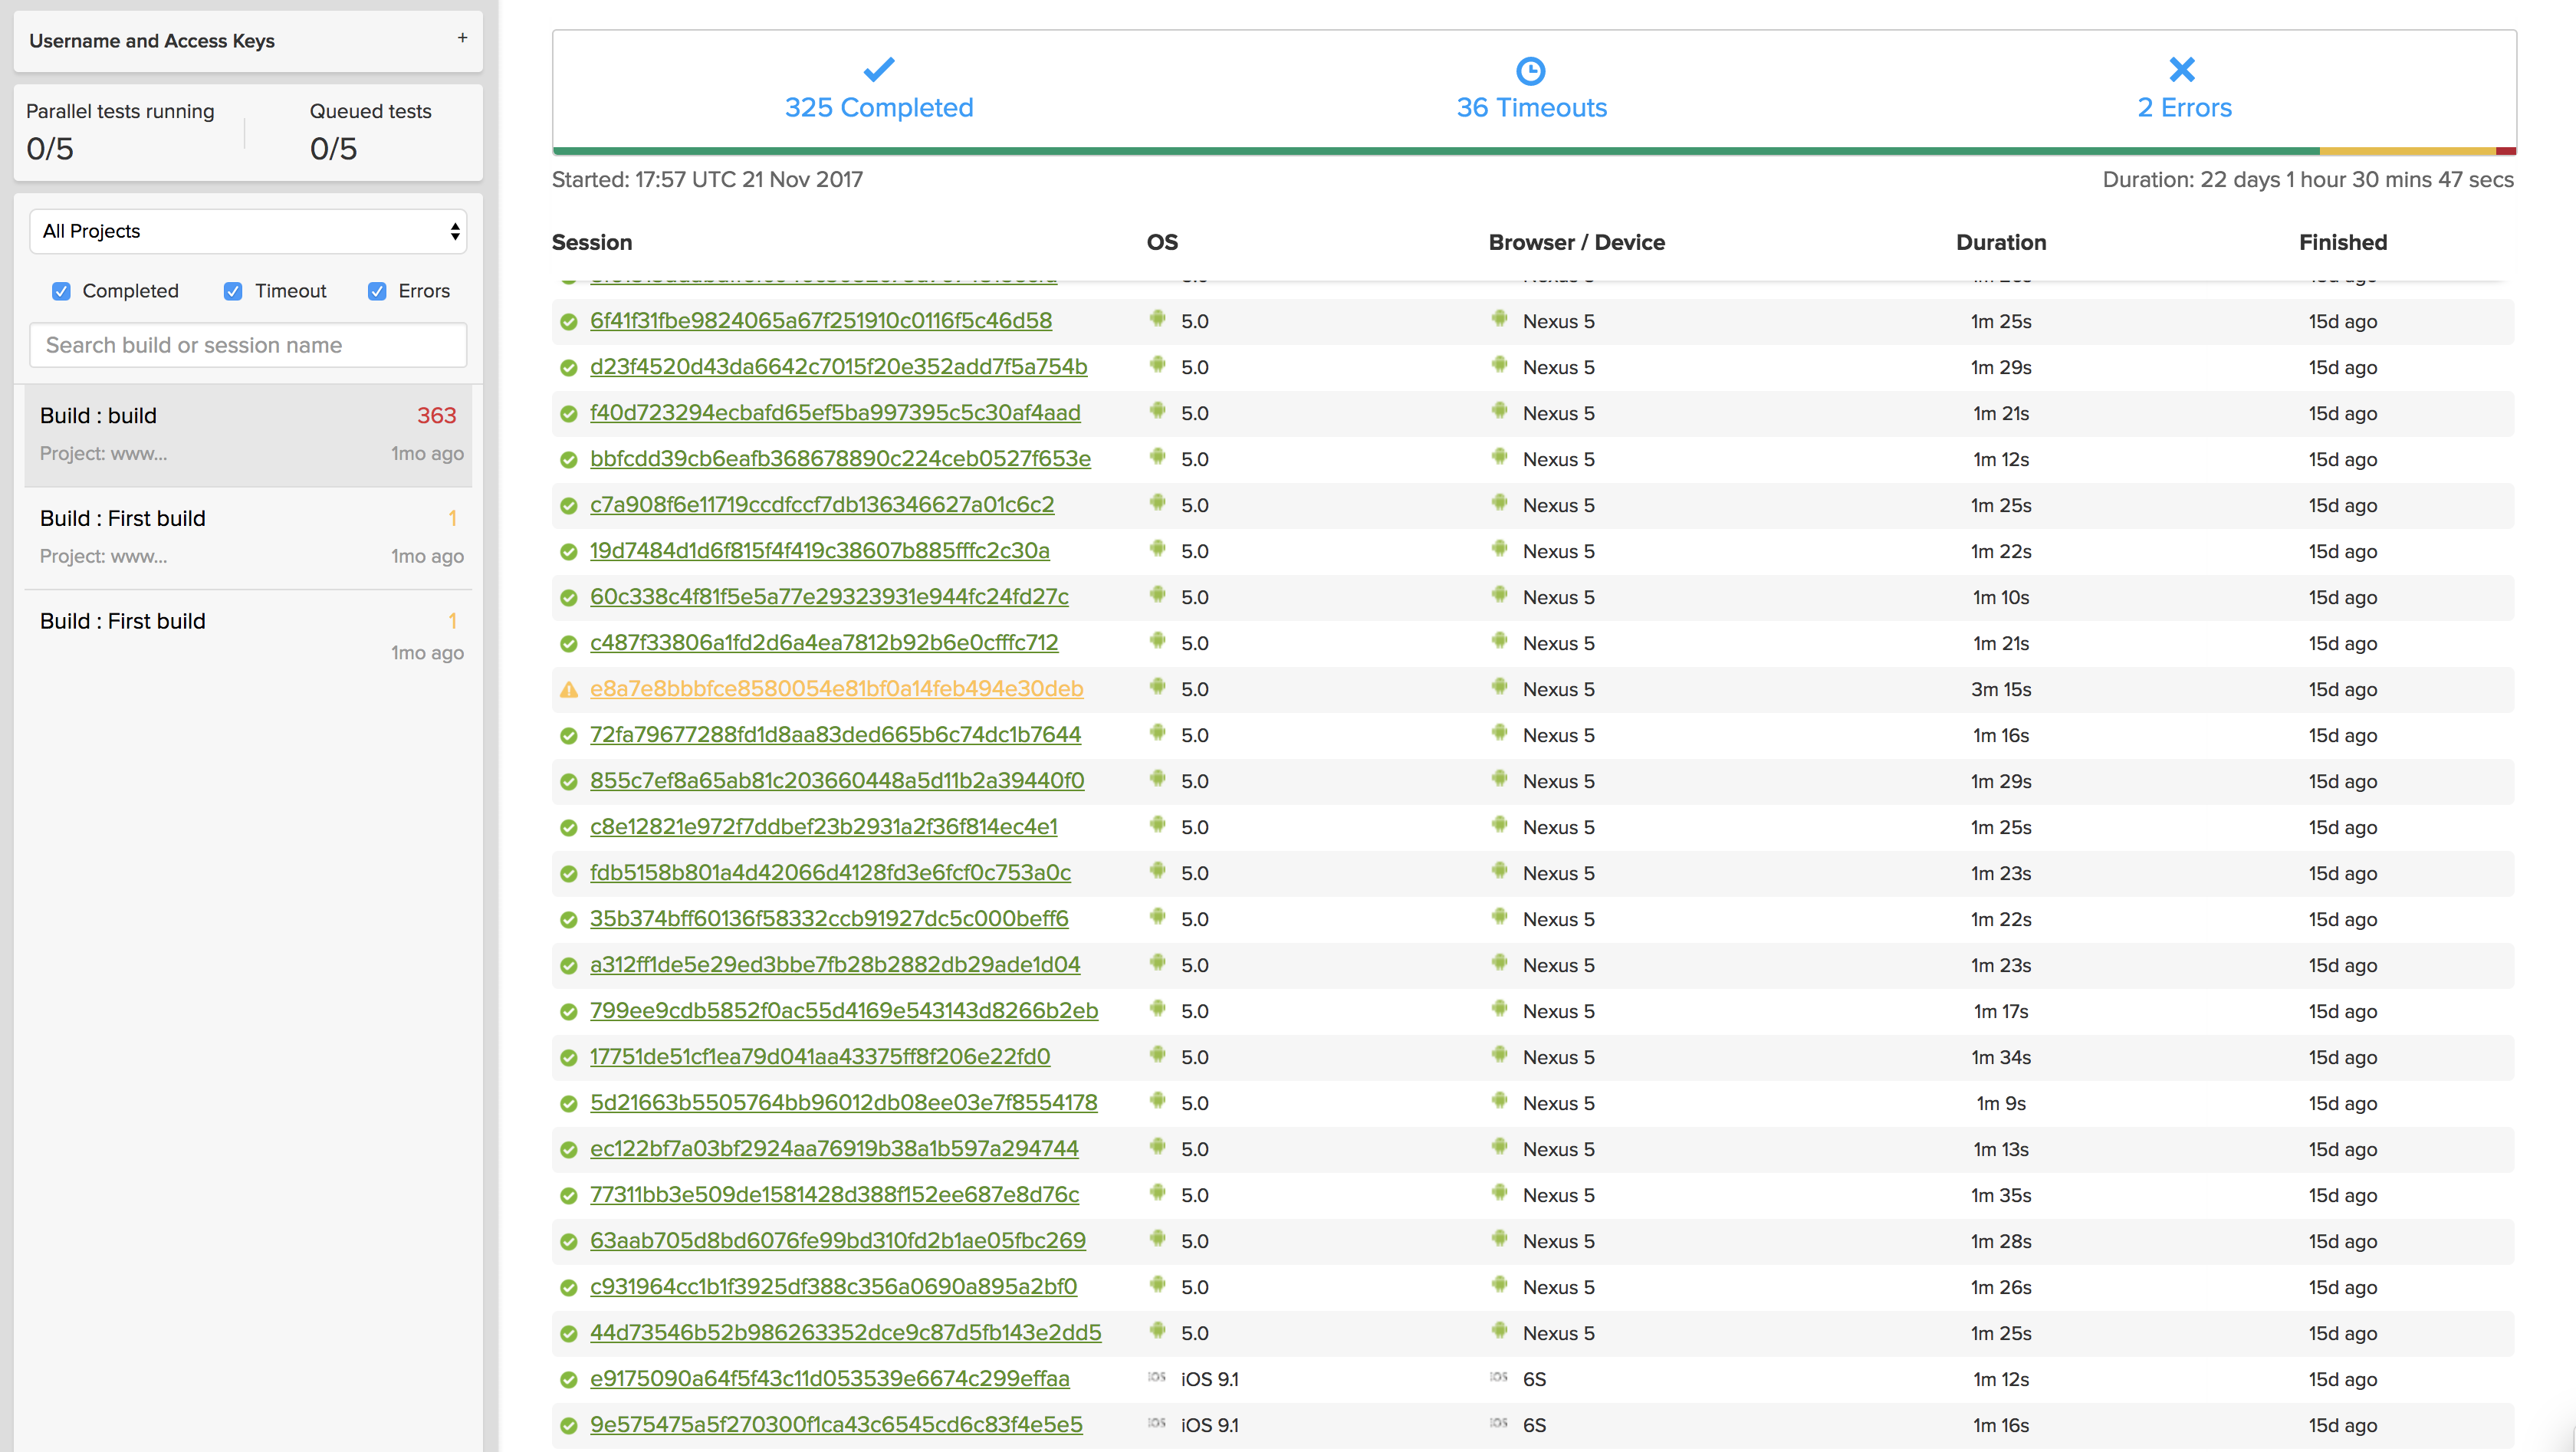
\includegraphics[width=\linewidth,keepaspectratio]{stack.png}
  \caption{Screenshot of BrowserStack dashboard}\label{stackpic}
\end{figure}

\begin{lstlisting}[caption={Measurement data example},label=mongodata, basicstyle=\scriptsize]

{
  "_id" : ObjectId("5a1c3a5bcf7b3443d70c4b34"),
  "browser" : {
    "family" : "Chrome",
    "major" : "62",
    "minor" : "0",
    "patch" : "3202"
  },
  "device" : {
    "family" : "Other",
    "major" : "0",
    "minor" : "0",
    "patch" : "0"
  },
  "os" : {
    "family" : "Mac OS X",
    "major" : "10",
    "minor" : "13",
    "patch" : "1"
  },
  "type" : "JS",
  "data" : {
    "sorting" : 0.10500000000001819,
    "size" : 50,
    "type" : "JS"
  }
}
\end{lstlisting}

For running different benchmarks on combinations of various different
devices and browsers, we set up an account on the popular browser testing
service BrowserStack. BrowserStack is originally meant for writing and running
end-to-end test cases for web applications, but for our purposes it fit our
needs perfectly. BrowserStack offers a simple API for programmatically
operating a given browser, and waiting for a certain condition to be fulfilled,
so the core testing code was only 20 lines of JavaScript or so. The testing
code can be in listing~\ref{stacktest}. In it, we simply iterate over the
various browsers, our test cases and their various parameters and launch an
asynchronous BrowserStack session for each of them. BrowserStack were also
extremely generous in offering us their paid services for absolutely no cost,
and we would very much like to extend our thanks for that.

\begin{lstlisting}[caption={BrowserStack testing code},label=stacktest, basicstyle=\scriptsize]

for (const c of capabilitiesUsed) {
  for (const p of projects) {
    for (const params of p.parameters) {
      for (t of p.testsAvailable) {
        console.log(
          `Running test ${p.name} ${t} on browser ${
            c.browserName
          } with query parameters ${params}`
        );

        const url = `${baseUrl}/${p.name}/${t}/?${params}`;

        doRun(url, c);
      }
    }
  }
}
\end{lstlisting}

All in all, we chose to test on nine different browsers. For all nine, we used
the latest available version on BrowserStack.

\begin{itemize}
  \item Internet Explorer 11
  \item Safari on macOS
  \item Opera
  \item Edge
  \item Safari on iPhone
  \item Safari on iPad
  \item Android default WebView browser
  \item Firefox
  \item Chrome
\end{itemize}

\section{Results}

Looking at the final results, our initial expectations were proven to be
correct. Across all supported browsers WebAssembly was the fastest, with asm.js
not too far behind. Native JavaScript and gpu.js were the slowest, as is to be
expected. For sorting and matrix multiplication, for asm.js and JavaScript it
made no difference if the data type being operated on was a float or double.
However, for WebAssembly operations were clearly faster on 32-bit integer data
types than for the other data types. For example, on Chrome sorting a list of
10000 random items took 10 milliseconds on average, 12 milliseconds for 32-bit
floats and 17 milliseconds for 64-bit doubles.

Across all platforms, WebAssembly was the fastest on Chrome and Firefox, and
slowest on Edge and Android WebView. For the sake of comparison, sorting 100
numbers took about 10 milliseconds on WebAssembly for floats on an Android
device using it's own WebView, while it only took about 0.5 milliseconds on
Desktop Chrome.

Asm.js was quite a lot faster on Firefox than other browsers. For example, for
multiplying two 1000 by 1000 matrices of random floating point numbers, it took
about 5290 milliseconds on Firefox for asm.js, while it took around 14520
milliseconds on Chrome, almost three times longer.

For matrix multiplication, gpu.js seems quite slow. For example, for the aforementioned a square
matrix of size 1000 \times 1000 gpu.js with another, on Chrome it took 43130
milliseconds for gpu.js, but just 14960 milliseconds for plain JavaScript. For
contrast, WebAssembly took just 2680 milliseconds, and asm.js took 14520
milliseconds.

\section{Analysis \& Conclusions}
As specified in the previous chapter, for all intents and purposes,
WebAssembly was indeed by far the fastest method for all three benchmarks on
all browsers. However, for the sake of fairness for WebAssembly and asm.js we
included not only the actual time spent on computations, but also the time
spent on passing data and dynamically managing memory. This overhead made WASM
and asm.js somewhat slower than native JavaScript on very trivial amounts of
data.

Asm.js came in second when it came to pure speed. On some browsers, mostly
Firefox, almost beating WebAssembly in some use-cases. It makes that asm.js
would be the fastest of Firefox, both technologies being made by the Mozilla
corporation. Firefox most likely has some asm.js specific optimizations in
place. In some ways it feels like asm.js is already somewhat outdated
technology currently. We see no reason one should use it if WebAssembly is a
viable option. Asm.js can still be used as a fallback for older browsers,
however, so it retains it's usefulness to that extent.

Using gpu.js to offload the easily parallelized matrix multiplication to the
GPU instead of the CPU was an interesting experiment. However, as is to be
expected there was a large overhead in moving data from the CPU to the GPU
pipeline, and then back again. To make matters worse, WebGL has no easy way of
passing simple numerical data back and forth like with regular OpenGL and the
CUDA toolkit. Instead, numerical data has to be first converted into a 2D
texture which must be loaded into WebGL before any operations can be performed
on it, and then it must be converted back before it can be used on the web
application side. The debugging tools were also very lackluster for gpu.js, and
we would not consider it production-ready in its current state. It was an
interesting experience none the less.

For us, using BrowserStack for automated testing was a good idea and a learning
experience, but debugging potential failures was somewhat difficult. For some
devices and test runs, it would occasionally crash without giving a clear
explanation as to why. If more accurate results were to be gathered, we would
suggest running thousands of tests more on real-world devices by hand, instead
of attempting to automate it. However, we would still recommend BrowserStack
for end-to-end testing of web applications, which is it's main purpose.

WebAssembly has recently gained support in all the latest
browsers~\footnote{\url{https://blog.mozilla.org/blog/2017/11/13/webassembly-in-browsers/}},
and we predict that it will continue to grow as the ecosystem and tooling for
it matures. During our tests, we ran into some issues of lackluster
documentation, but that will not be an issue once adaption rate increases.
Besides the performance implications, we feel that the breakthrough factor that
will make WebAssembly succeed in the long run is the fact that one no longer
has to write their web applications in JavaScript, but can choose from any
number of other languages without the inevitable legacy baggage that comes with
JavaScript, since the EcmaScript standard has to stay backwards compliant for
the unforeseeable future. Currently, the biggest hurdle for WebAssembly is the
lack of DOM operations and the lack of a standardized garbage collector, but
those are currently being worked on. All in all, we believe that in the coming
years writing "plain" JavaScript will become more and more rare, as
intermediate formats and compilers like WebAssembly and
Babel~\footnote{\url{https://babeljs.io/}} become more and more widespread. Of
course, JavaScript itself is not going anywhere soon, but it is our belief that
it and its interpreters will become more of a virtual machine for running code
on the browser, than a programming language unto itself.

\bibliographystyle{IEEEtran}
\bibliography{report}

\end{document}

